\documentclass[a4paper]{article}

\setcounter{secnumdepth}{3}
\usepackage[english]{babel}
\usepackage[utf8x]{inputenc}
\usepackage{amsmath}
\usepackage{url}
\usepackage{graphicx}
\usepackage{fixltx2e}
\usepackage{color}
\usepackage[colorinlistoftodos]{todonotes}
\usepackage{array}

\title{Classification of Wikipedia articles using natural language processing}
\author{
  Berenji, Sarah\\
  \texttt{sarah.berenji@gmail.com}
  \and
  Forsten, Andreas\\
  \texttt{andreasforsten@gmail.com}
  \and
  Leskelä, Hannes\\
  \texttt{hleskela@kth.se}
  \and
  Letzner, Josefine\\
    \texttt{joletzner@gmail.com}
}
\date{2015-10-04}
\begin{document}
\maketitle
\begin{abstract}

\noindent In this project we have developed two different text analysers focusing on categorizing the content of Wikipedia articles. One analyser was based on Naive Bayes and the other was built on reinforcement learning techniques. The train and test datasets consisted of Wikipedia articles which were gathered with the aid of Blockspring and the Wikipedia API. The results showed that both Naive Bayes and the Reinforcement learning approach worked well for classifying articles but that the Naive Bayes might be faster and in need of less training data in this specific case.
\end{abstract}
\newpage
\tableofcontents
\newpage

\section{Introduction}


\noindent The first section of this paper describes the aim of the project. After a discussion about the different existing methods for NLP in section 2, we provide our method and the tools we are going to use. A summary of the results is provided in section 4, and then a brief discussion of them finishes the paper in section 5.
\vspace{3mm}

\subsection{Objective}
 
Text analysis as a discipline has been around for decades, and the growing need for handling large amounts of unstructured data means that the relevance of the discipline is ever growing \cite{HistoryofTextAnalytics}. As an example, it is estimated that 62 billion e-mails are sent per day, and every day searchable web sites add enough information to fill millions of books \cite{ChallengesInTextAnalytics}. Handling the challenge of the surge of information caused by the arrival of the Internet spawned many new techniques for doing analysis, and in this paper a case study of the subject is done with the aid of \textit{Wikipedia}. 

\vspace{3mm}

\noindent As of today (October 2015), almost five million articles have been published on the English version of Wikipedia\cite{wikipedia}. The articles are sorted in categories and so-called portals, which mean that they provide a good opportunity for testing text analysis techniques on large amounts of data. By using \textit{SciKit-learn} and \textit{TextBlob}, which is built on top of the \textit{Natural Language ToolKit} (\textbf{NLTK}) and \textit{pattern}\cite{textblob}, an attempt to correctly assign categories to Wikipedia articles was made, with results analysed and discussed in this paper. 

\vspace{3mm}

\subsection{Problem Statement}

\vspace{3mm}


- What techniques are well suited to the problem of text categorization? What are their respective advantages and disadvantages?

\vspace{3mm}

- What are the difficulties in text categorization? Are certain texts harder to correctly categorize than others, and if so, why?


\vspace{3mm}


\section{Background}

\vspace{3mm}

The problem of trying to categorise texts based on their content is a problem in the field of \textit{Natural language processing} (\textbf{NLP}). NLP focuses on the questions on how to make computers interact with human language in one way or another.\\

\noindent Exactly how far the history of NLP stretches back in time is a matter of debate, but many would say that is starts around 1950 when Alan Turing published an article in which he proposed the "Turing test", which did not actually say much about NLP, but set a criterion for computer intelligence which is used until this day \cite{AI}. To pass this test a computer has to pass as a human after being interrogated by a person. Many methods for solving these kind of problems have been tried and numerous people have contributed to the knowledge we have about NLP today. In the late 1980's NLP as a discipline saw something of a revolution \cite{historyNLP}. At this point the computational power had become sufficient enough to use machine learning to solve NLP problems. In what follows some different methods are briefly over-viewed and how they apply to the specific questions stated in this report.\\

\noindent Maybe the most intuitive and simple way of dealing with the problem of text classification is to view it as a \textit{data compression} problem. Even though it may seem as if words can be combined in an infinite number of ways, there are often recurring patterns that can be recognized \cite{AI}. Storing patterns will eventually end up in a language model \cite{ColumbiaUniversity} which is a probability distribution over a sequence of words. With the computational power available today it is not reasonable to try to store all these patterns without processing, since they can contain several tens of thousands of words or more. The solution to this is to compress the data. There are different algorithms for doing this. Two commonly used are the \textit{Lempel-Ziv-Welch-algorithm} (\textbf{LZW}) and \textit{Huffman}\cite{handouts}. A LZW compression algorithm takes each input sequence of bits and creates an entry in a table for that particular bit pattern, consisting of the pattern itself and a shorter code. As input is read, any pattern that has been read before results in the substitution of the shorter code, effectively compressing the total amount of input.\\One advantage of this approach is its simplicity. However, there are several drawbacks apart from the need of memory in order to get a decent dictionary; slow running times being one\cite{hstein}. \\

\noindent Another method which will not be mentioned much here but more in the chapter "method", as this was the method chosen for solving the problem stated in this report, is the machine learning based approach. There are numerous ways to implement this, but to summarise them they are probabilistic algorithms that can be trained in different ways (e.g. supervised, or unsupervised) so that they can later recognise handle data that they have not previously processed already. A family of such algorithms go under the name of Naive Bayes. What these have in common is that they assume independence between features. This makes it possible to calculate the probability of events separately, and with these probabilities the joint probability of the separate events is found, and the option which has greatest probability is chosen.



 


\section{Method}  

\noindent Python was the programming language of choice for this project. For classification, noun extraction and other natural language processing techniques TextBlob and SciKit-learn was used. Data was obtained with the wikipedia API and Blockspring. In this section we provide a brief overview of these tools, and how we used them.

\subsection{Tools}  
\subsubsection{TextBlob}

TextBlob is an open source Python library for performing simple language processing tasks. Textblob provides a simple API for common natural language processing (NLP) tasks. This library inferres underlying structures of the text's language available to computer programs for analysis and manipulation. It was used mainly for its noun extraction feature.

\subsubsection{Using TextBlob}

The basic steps to use TextBlob are:

\begin{itemize}  
\item Creating a TextBlob object. This object takes the text - which we want to work with - as a string type.
\item Use various methods of this object to process the text.
\end{itemize}

A TextBlob object provides several different methods that can help us to categorise and analyze a text. Here some of these methods are described briefly to show how TextBlob can be used to process the text. 

\textcolor{red}{To Hannes and Sarah: What parts of this should be left? Is all of this used?}
\begin{description}
  \item[Tokenization (sentences, words and noun phrases)] \hfill \\
  The resulting TextBlob object has \texttt{.sentences} method that lists all the sentences in the text. It is possible to take the words from each of the sentence objects by using \texttt{.words} method. There is also the \texttt{.noun\_phrases} method of TextBlob object that returns the text of all noun phrases found in the text.
  
  \item[Part-of-speech tagging] \hfill \\
  The \texttt{.tags} method of TextBlob object can tell us what parts of speech each word in a text corresponds to. In the resulting output, it tags different words of the text with their role in the sentence using the following tags: 

  NN: noun

  JJ: adjective

  IN: preposition

  A more complete list of tag meanings can be found on the CLiPS  \footnote{http://www.clips.ua.ac.be/pages/mbsp-tags} website.
 
  \item[Word inflection] \hfill \\
  TextBlob library has another object called \texttt{Word}. This object can be used for pluralization, singularization and lemmatization of a word. For example the Word object provides \texttt{.pluralize()} method which takes a single word and returns the plural form of that word. 
 
\end{description}
Some of the other features of TextBlob library are:
Sentiment analysis: .sentiment
Classification (Naive Bayes, Decision Tree)
Language translation and detection powered by Google Translate
Word and phrase frequencies
Parsing
n-grams
Spelling correction
Add new models or languages through extensions
WordNet integration


\subsubsection{SciKit learn} 

\label{sec:sklearn}
The TextBlob Naive Bayes classifier was used at first, but turned out to be too slow for our purposes. We tried building classifiers with whole texts as train data, but as it performed poorly we changed to using just article nouns. The Multinomial Naive Bayes (henceforth abbreviated MNB) classifier of SciKit-learn (henceforth abbreviated sk-learn) was then used instead, which performed significantly better. To perform the classification one has to use a vectorizer which transforms the data from text to a matrix, which was done by the built-in CountVectorizer. We decided to use the TfIdfVectorizer for feature extraction, where TfIdf referrs to the tf-idf transform or \textit{term-frequency - Inverse-document-frequency} transform\cite{skfeatures}. This transform is combined with the CountVectorizer to form the model that is the TfIdVectorizer.\\

\noindent By term frequency we mean that the importance of a word in a document is proportional to its frequency of occurence, which is often called Luhn's assumption\cite{luhn}. To complement this one may add the inverse document frequency factor to the model, which gives more importance towards less commons words in the document as well. This was conceived by Spärck\cite{sparck}, and may be summarised as:\\
\\
\textit{The specificity of a term is inversely proportional to the number of documents in which it occurs.} \\

\noindent This means that weight will be given to words that occur more in some specific documents.\\

\noindent There are several parameters which may be given as arguments to the TfIdfVectorizer. The ones used in this paper are \textit{minimum document frequency}(min\textunderscore df), \textit{maximum document frequency}(max\textunderscore df) and \textit{Top maximum features}(max\textunderscore features).
The minimum document frequency is, as its name suggests, the threshold on how few documents a term may occur in before it is ignored. Setting this to one is the same as not ignoring any terms at all.
The maximum document frequency is the reverse of this; the threshold on how many documents a term may occur in before it is ignored. If the top maximum features parameter is specified, only the top most frequent terms will be taken into account when classifying.


\subsubsection{Blockspring and the wikipedia API}

In order to gather a dataset as an input to TextBlob and consequently SciKit, we used Blockspring. Blockspring has the ability to get articles belonging to specific Wikipedia categories and subcategories, which we used as our input dataset. It has different blocks for getting information from Wikipedia pages. First one chooses the different categories one wants, such as physics, history or medicine. Then we used the "Get Wikipedia Sub-Categories" block from Blockspring to get the Wikipedia sub-categories of our selected categories. The original plan was to use Blockspring to retrieve the articles themselves as well, but as it had problems doing so without errors we got the content of the articles with an API called wikipedia instead. 




\subsection{Classification methods}
\subsubsection{Naive Bayes} 

Naive Bayes is a simplified version of Bayes theorem, where the denominator is considered redundant since\
 it doesn't give us any information about the action we've looking for. So Bayes theorem can be simplified to the joint probability model as follows:
\\\[p(C_k|x) = \frac{p(C_k)p(x|C_k)}{p(x)} \Longrightarrow p(C_k)p(x|C_k) = p(C_k,x_1,x_2,...,x_n)\]\\
This in turn, using the chain rule, would yield us the series of probabilities \[p(C_k,x_1,x_2,...,x_n) = \]
\[p(C_k)p(x_1,x_2,...,x_n|C_k) =\]
\[p(C_k)p(x_1|C_k)p(x_2,...,x_n|C_k, x_1) = ... =\]
\[p(C_k)p(x_1|C_k)p(x_2|C_k, x_1) ... p(x_n|C_k, x_1, x_2,...,x_(n-1) \]\\
Now, if we assume that each individual action is independent, which is the naive part of naive Bayes, and given the category $C_k$, we can write the probabilities as s\
imply $p(x_i|C_k, x_j,x_k...) = p(x_i|C_k)$. In our case, we can think of this as the probability of a word being in a text, given the category C, is strictly a matter\
 of how often the word has occurred in such a category in our training. Then, the category will be determined by a predetermined set of keywords and their occurrence 
rate for the category.\\

\noindent In this paper multinomial Naive Bayes was used, which is one of the two classical implementations of Naive Bayes (the other being Bernoulli Naive Bayes). The word multinomial referrs to the fact that we have a multinomial distribution, where each event is the occurrence of a word in a single document.\\

\noindent Naive Bayes has been shown to work quite well despite its assumption of independence. The reason for this is that the dependencies tend to cancel out\cite{NBindependence}. 

\subsubsection{Reinforcement Learning}
Besides using the built-in Naive bayes method, a simple version of reinforcement learning is implemented to determine if the naive approach is indeed too naive. The pr\
imary choice of method is Reinforcement Learning (RL), since we have some knowledge of this algorithm from a previous course. When constructing a reinforcement based a\
lgorithm, it is of great importance to choose a good heuristic for determining the category, and also a grading heuristic to accompany this heuristic. The grading heur\
istic is basically a formula with fixed variables but varying multipliers for the variables. RL then aims to maximize the ``score'' when categorizing text based on the\
 heuristic that scores a result. Then you edit one of the multipliers with a fixed, small value until a maximum result is found. You then iterate over the variables, i\
ncrementing them slightly trying to find the best categorizer is created. The problem is that you cannot be sure that the maximum result is a local or a global one, wh\
ich means that you need to make drastic jumps from time to time to try and find a better value. This method is quite time consuming but can possibly yield a better res\
ult than the Naive Bayes method, depending on how good our heuristic is.

\section{Results}

\subsection{Multinomial Naive Bayes with SciKit}

A varying number of articles were classified in one of nine categories: \\
Physics, Mathematics, Medicine, History, Sports, Psychology, Philosophy, Computing and Biology.\\
\subsubsection{min\textunderscore df, max\textunderscore df and max\textunderscore features}
\label{sec:parameters}
For information about min\textunderscore df, max\textunderscore df and max\textunderscore features referr to section \ref{sec:sklearn}.

\noindent The tests in this section was done with a sample of twenty-five articles from the above specified categories.
\noindent The results for the MNB with min\textunderscore df $= 1$ with varying train data size can be seen in figure \ref{fig:MNB_first} (note that min\textunderscore df $= 1$ is the default value for the vectorizers, and it does not exclude any words based on document frequency). 
\begin{figure}[h!]
  \centering
    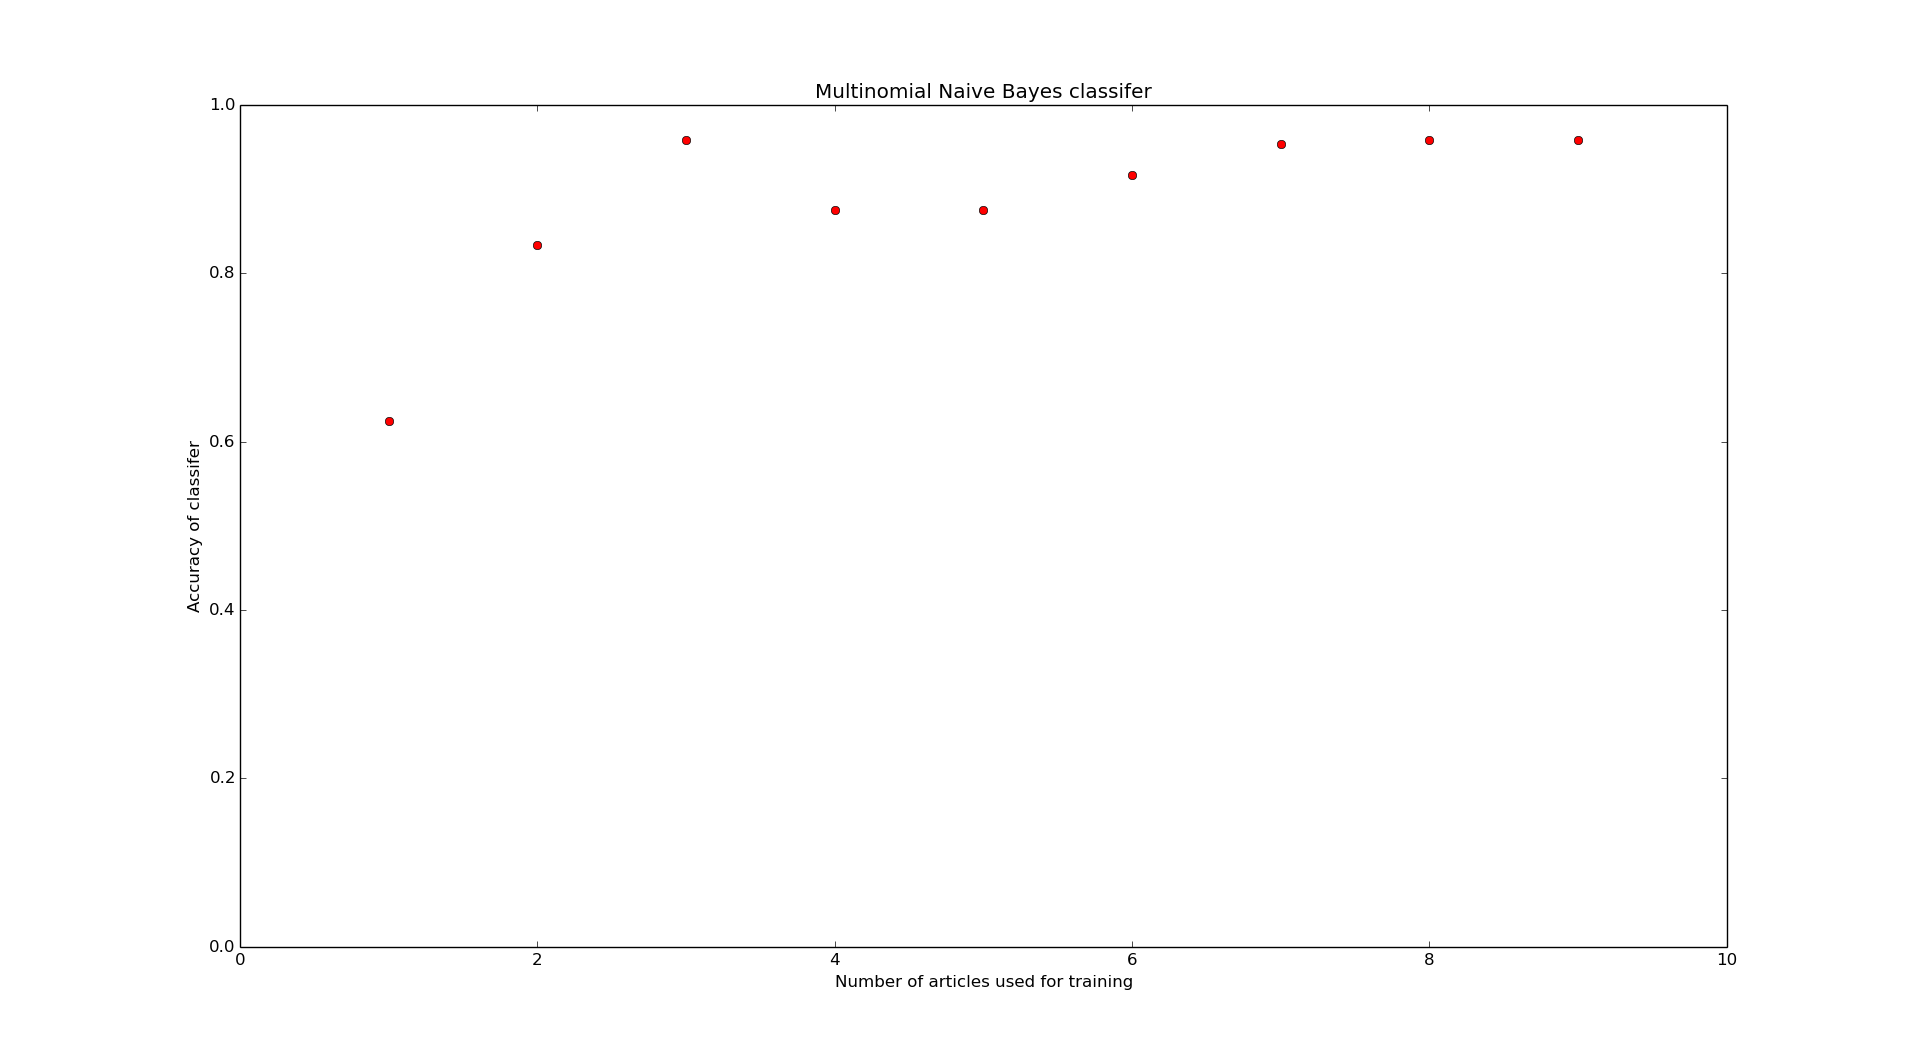
\includegraphics[width=1.0\textwidth]{MNB_first}
  \caption{Variations in performance based on training size, min\textunderscore df $ = 1$}
  \label{fig:MNB_first}
\end{figure}
\vspace{3mm}

\noindent With max\textunderscore df = 1, see figure \ref{fig:MNB_second}

\begin{figure}[h!]
  \centering
    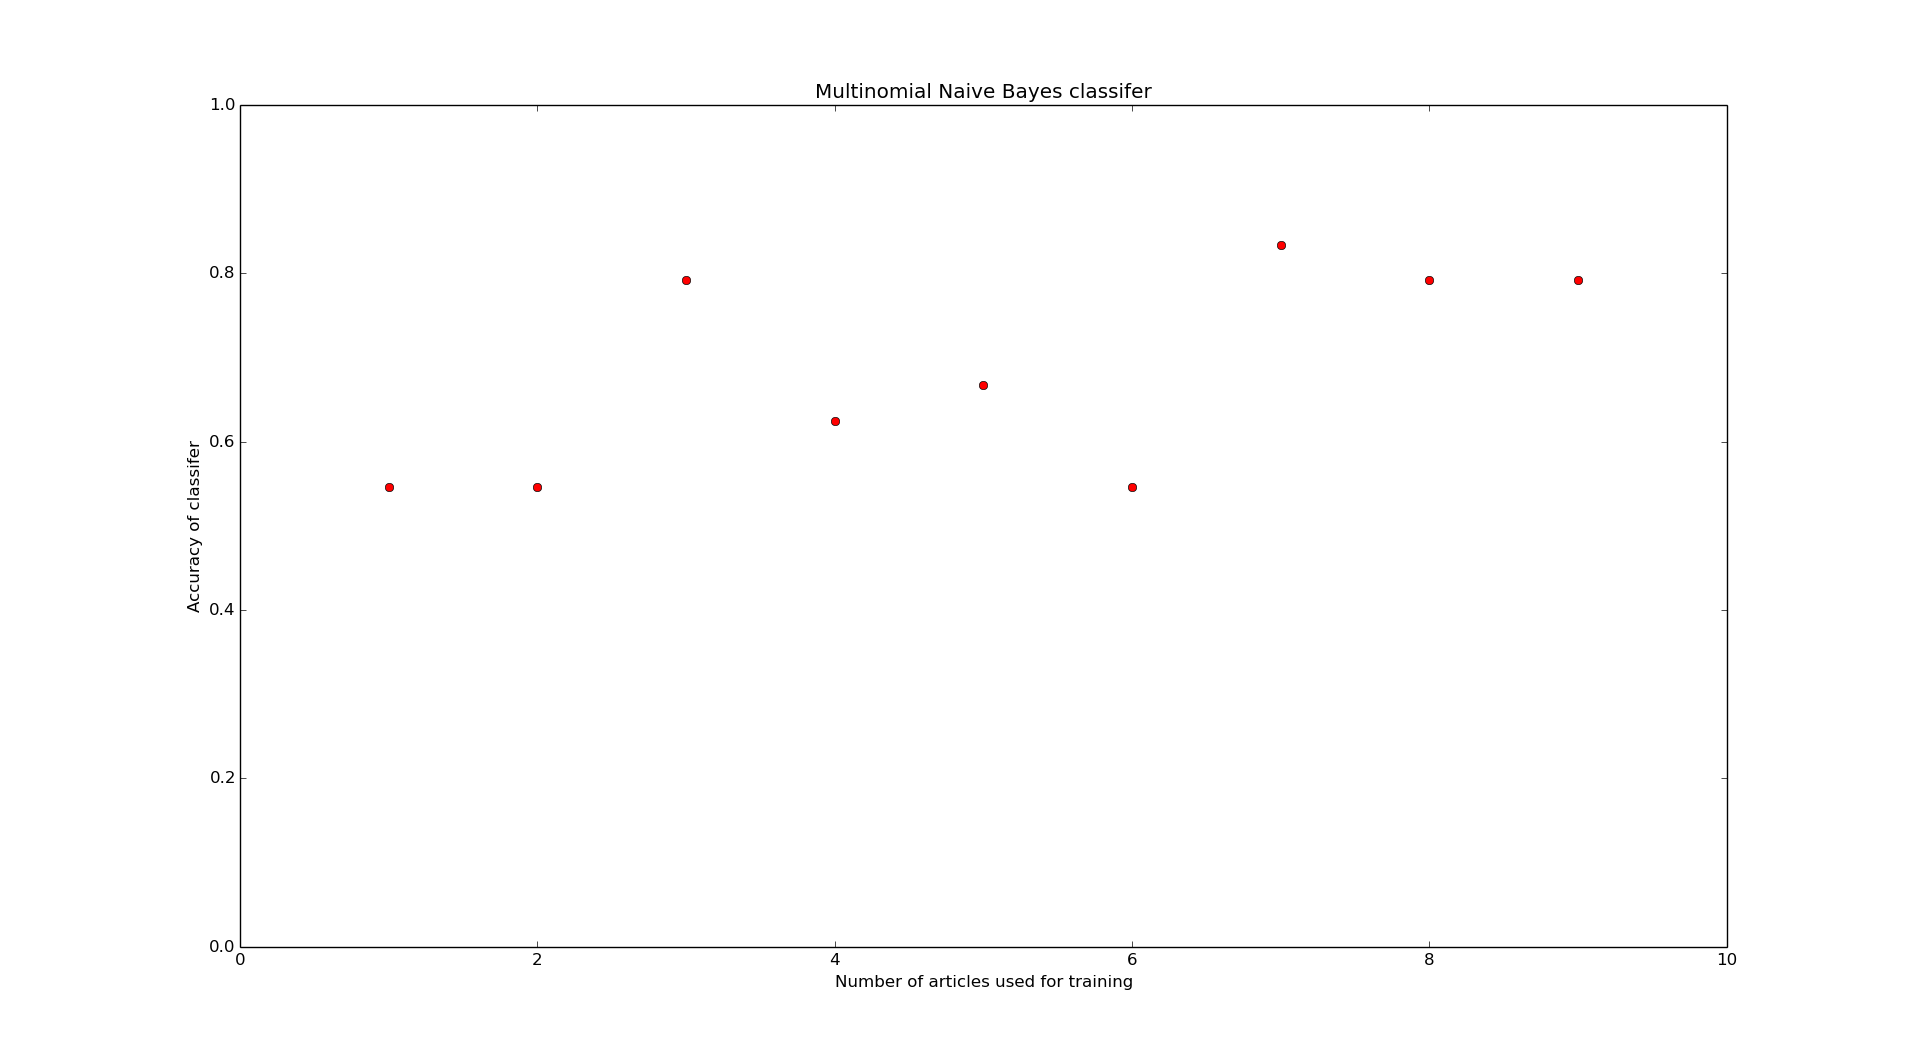
\includegraphics[width=1.0\textwidth]{MNB_second}
  \caption{Variations in performance based on training size, max\textunderscore df $ = 1$}
  \label{fig:MNB_second}
\end{figure}

\noindent With max\textunderscore features varying between 1 and 300, see figure \ref{fig:MNB_third}.

\begin{figure}[h!]
  \centering
    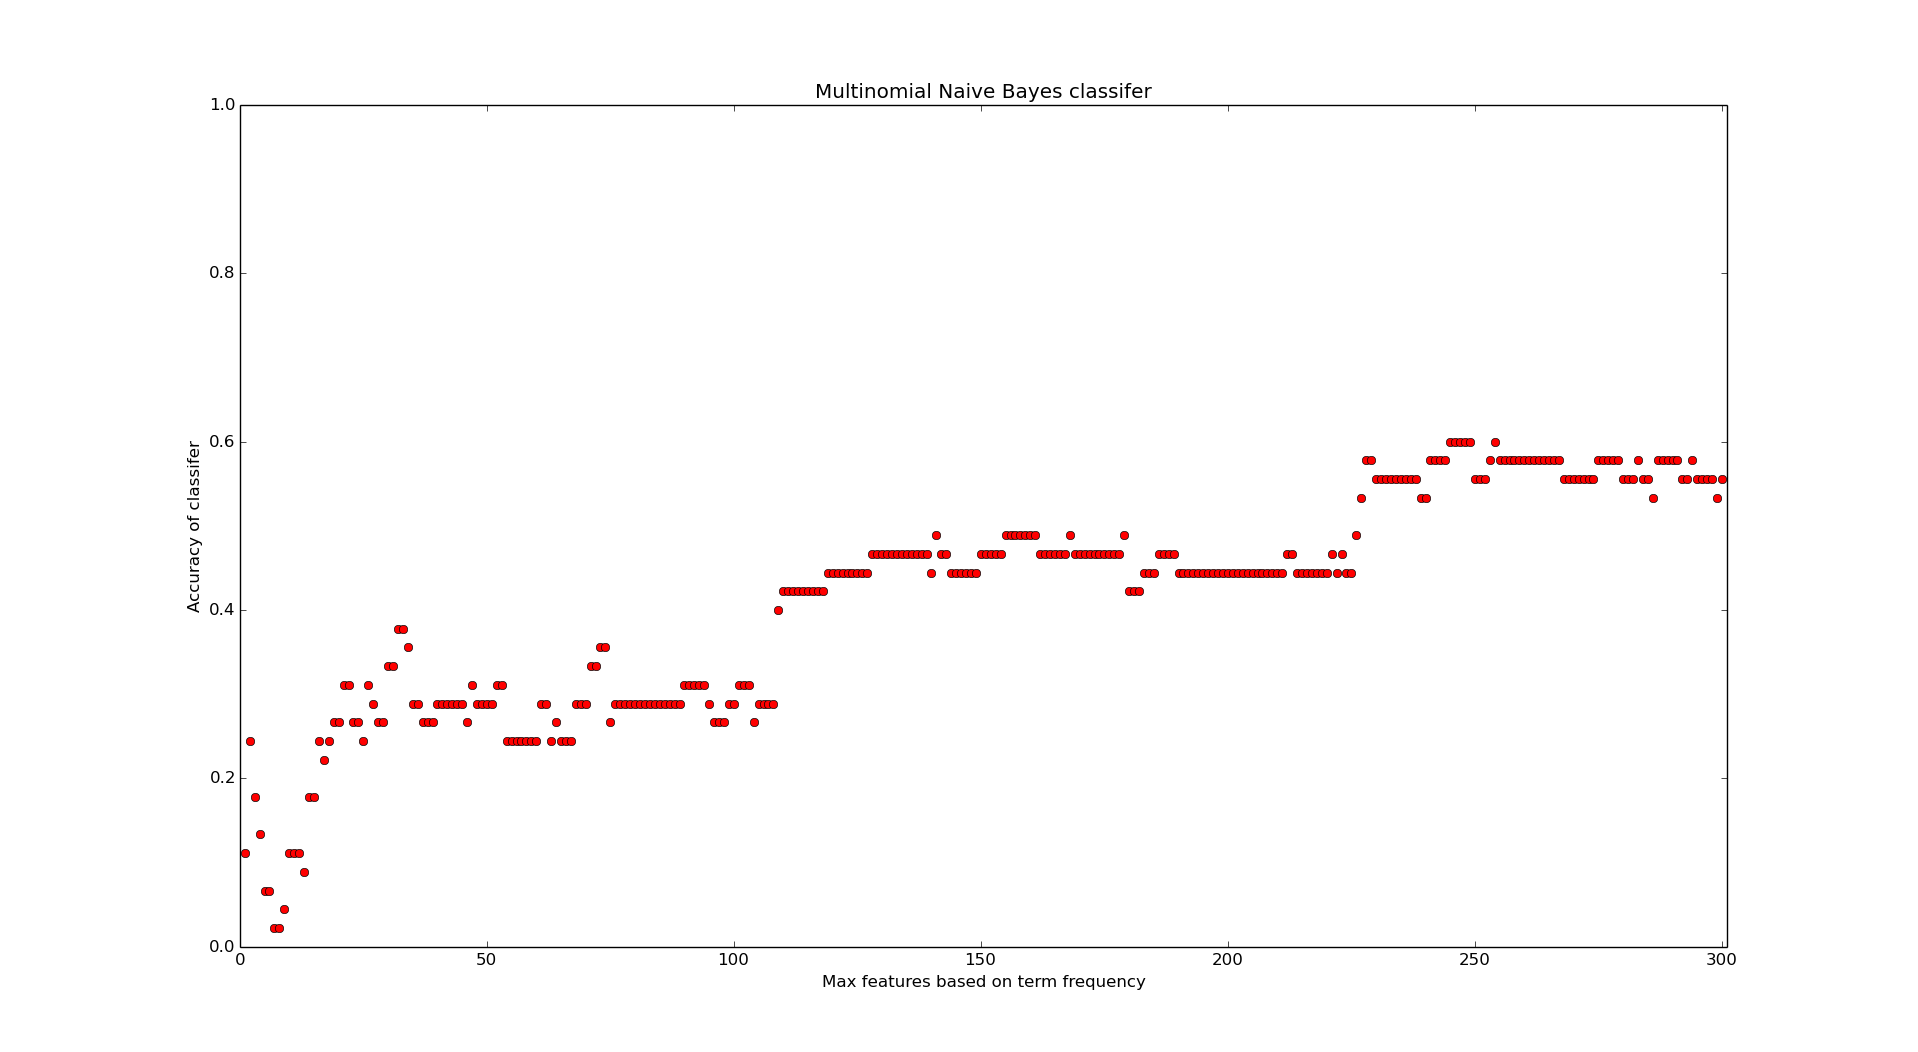
\includegraphics[width=1.0\textwidth]{MNB_third}
  \caption{Variations in performance based on training size, max\textunderscore features varying between 1 and 300.}
  \label{fig:MNB_third}
\end{figure}

\subsubsection{Variations in test and train data size}

\noindent The train data was changed to five articles from the main categories above, and two articles from each of their subcategories. max\textunderscore features was not used, min\textunderscore df was set to one.\\

\noindent First, the test data was increased from 25 articles to 45 articles. The MNB trained with the new data had an accuracy of 100\% on these.\\

\noindent The test data was then changed to very short biology articles on Wikipedia. First, ten articles with byte length shorter than three thousand bytes were tested, and the classifier had an accuracy of 80\% on them. When the byte length was increased to five thousand the accuracy went up to 100\% again.
\noindent The data on byte length was gathered from wikipedia.\footnote{\url{https://en.wikipedia.org/wiki/Wikipedia:Short_popular_vital_articles}}


\section{Discussion}

\subsection{The Multinomial Naive Bayes classifier}



The parameters in section \ref{sec:parameters} were tested to find out the optimal way to classify our articles. Setting min\textunderscore df to one and ignoring the max\textunderscore features, which takes into account all terms in the corpus, proved to be superior to the other alternatives. In figure \ref{fig:MNB_first} we see that improvement in capacity is not necessarily correlated with training data size. This is natural when one considers that the training data only consisted of nouns. If the MNB is to classify articles correctly, it will have to find words in its own article that are the same as in the training data of the correct category. To construct a well performing classifier it is then more important to have varying data than lots of it, even though the amount does of course matter in some cases due to term frequency being a factor.\\

\noindent The classifier performed varyingly, but less well, when the maximum document frequency was specified. It might seem that it should perform well if only terms that are unique to a category are used. This might be because common key terms are excluded. For example, 'mathematics' may be a key word in identifying mathematics articles. But if it occurs once in the physics training data it would be excluded. This is an unnecessary loss of information, and it might be the reason for it performing less well. \\

\noindent Tests were then done on smaller articles, but as the main difficulty of our classifier is not article length but differences the nouns used compared to the training data, the classifier still performed quiet well. For example, 'Myrtales' and 'White Currant' has an approximately equal byte length (at the date of retrieval, October 2015), and both of them are flower articles. Our classifier did not classify 'White Currant' article correctly, but the 'Myrtales' article was correctly classified as biology. The reason is quiet obvious when one looks at their content. 'Myrtales' contains words such as 'DNA' and 'Gene' which occur frequently in all biology articles. 'White Currant' does contain the words 'species' and 'plant', but it also contains the words 'Iron', 'Copper' and 'Manganese', which might be the reason for it being classified as 'Computing'. Article length does matter, but mainly for the reason that there is a higher probability of these sorts of mistakes occurring.


\subsection{Comparison between Naive Bayes and Reinforcement Learning}

A strength of Naive Bayes is that it needs little training data\cite{NBtrainsize}. This was seen in the results, as it performed well even if only two or three articles were used for training. Another strength is that it is fast, as it assumes independence\cite{NBfast} of the words (each distribution is one-dimensional).\\

\noindent However, while Naive Bayes worked well for the classification done in this project, it might not perform well with other sorts of NLP problems, as it is known as a bad estimator. This means that the probabilites it assigns to its classifications are inaccurate, but it does not matter as long as the maximum probability is assigned to the correct category\cite{NBestimation}.\\

\textcolor{red}{To Hannes and Sarah: Is reinforcement learning better at estimation? What effect does this have?}

\textcolor{red}{To Hannes and Sarah: What differences exist in how we train the classifiers? In Naive bayes everything has to be done by hand. How is it with reinforcement learning?}

\noindent The efficiency of the reinforcement learning depends on its policy, which may require a lot of work to implement well. However, this also makes the method more dynamic than Naive Bayes, as it can handle more types of problems.

\textcolor{red}{To Hannes and Sarah: Something about reinforcement learning + HMMs? If you dare to answer their questions on it...}

\subsection{Further work}
Since the accuracy obtained by the Naive Bayes classifier was close to 100\% a natural extension of the project would be to try to categorize the articles in subcategories and evaluate performance. As the difficulty of the problem is increased the Naive Bayes classifier might also need to be improved. This could be done by investigating what other relevant features of a text there are except nouns, or to use more varied train data. 

\subsection{Conclusion}

Naive Bayes with nouns as training data seems to work well for this problem, as it correctly classified articles almost 100\% of the times even with only a small training sample. However, it might not be well suited for other types of problems, such as classifying text type or classification within other types of texts\cite{NBpoems}. For these types of problems reinforcement learning might be more well suited, as it is more dynamic.
 
\begin{thebibliography}{9}

\bibitem{HistoryofTextAnalytics} 
Grimes, Seth. “A Brief History of Text Analytics”, b-eye-network, October 20, 2007.

\bibitem{ChallengesInTextAnalytics}
“Mastering new Challenges in Text Analytics”, IBM Business Analytics, May 2010, p. 1.

\bibitem{wikipedia}
\url{https://en.wikipedia.org/wiki/Wikipedia:About}. Retrieved 2015-10-04.4

\bibitem{textblob}
\url{https://textblob.readthedocs.org/en/dev}. Retrieved 2015-10-04.

\bibitem{AI}
Russell, Stuart. Norvig, Peter. "Artificial Intelligence, a Modern Approach" 3 ed. Pearson. p. 2.

\bibitem{historyNLP}
Lichtig, Ryan. "The history of Natural Language Processing". \textit{ETHW}. 

\bibitem{ColumbiaUniversity}
Collins, Michael. "Language modelling". Columbia University. 2013.


\bibitem{handouts}
"Compression Algorithms: Huffman and Lempel-Ziv-Welch(LZW)". (2012). MIT.
\url{http://web.mit.edu/6.02/www/s2012/handouts/3.pdf} Retrieved 2015-10-04.

\bibitem{hstein}
Marton et Al. "On Compression-Based Text Classification". 27th European Conference on Information Retrieval.


\bibitem{skfeatures}
\url{http://scikit-learn.org/stable/modules/feature_extraction.html}
Retrieved 2015-10-13.
\bibitem{tfidf}
Rajaraman, A, Ullman, J. D. (2011). "Data Mining". Mining of Massive Datasets. pp. 7-9.

\bibitem{luhn}
Luhn,Hans Peter (1957). "A Statistical Approach to Mechanized Encoding and Searching of Literary Information". IBM Journal of research and development (IBM) 1 (4): p. 315.


\bibitem{NBindependence}

Zhang, Harry (2004). "The optimality of Naive Bayes". University of New Brunswick. p. 1.


\bibitem{sparck}
Spärck Jones, K. (1972). "A Statistical Interpretation of Term Specificity and Its Application in Retrieval". Journal of Documentation 28: 11–21.

\bibitem{NBtrainsize}
Jin, David. Lin, Sally (2011). "Advances in Electronic Engineering, Communication and Management". Vol 1. p.337.

\bibitem{NBfast}
Zhang, Harry (2004). "The optimality of Naive Bayes". University of New Brunswick. p. 1.


\bibitem{NBestimation}
Ibid. p. 2.

\bibitem{NBpoems}
Mohammed, Iqbal.(2009). "Naive Bayes for Classical Arabic Poetry Classification". Journal of Al-Nahrain University. Vol. 12 (4). pp.217-225
\end{thebibliography}



%1. Artificial intelligence a modern approach, stuart russel
%2. $http://ethw.org/The_History_of_Natural_Language_Processing$ (måste förbättra källa?)



%We've chosen to do a version of the text analyser project, where we focus on categorizing either the content of the text or the type of text, depending on the difficulty level of the two alternatives. We will do this by implementing a heuristic that uses hidden Markov models, where we will research which variables should be included and give them a certain weight. If we have enough time, we will try to improve the heuristic by applying some sort of machine learning to the heuristic. If this is the case, it will probably be a simple version of policy gradient reinforcement learning (pgrl). We will work in python \textgreater= 3.0 and use some sort of natural language library to do the statistical analysis of the texts. Example libraries are TextBlob (https://textblob.readthedocs.org/en/dev) and the Natural Language Tool Kit (http://www.nltk.org)
%\newline


\end{document}
